\documentclass{article}
\usepackage[margin=1in]{geometry}
\usepackage{graphicx}
\usepackage{titlesec}
\usepackage{blindtext}
\setlength{\parindent}{0em}


\begin{document}

\titleformat{\section}
{\huge\bfseries}
{}
{0em}
{}[{\titlerule[1.5pt]}]

\titleformat{\subsection}
{\Large\bfseries}
{}
{0em}
{}

\begin{titlepage}

    \begin{center}

    \begin{figure}
    \centering
    
\includegraphics[height=3in]{bracu_logo.png}
    \end{figure}

    \end{center}



    \begin{center}

    \rule{\textwidth}{1.6pt}\vspace*{-\baselineskip}\vspace*{2pt} % Thick horizontal rule
	\rule{\textwidth}{0.4pt} % Thin horizontal rule
	
	\vspace{0.75\baselineskip} % Whitespace above the title
	
	\bfseries{\LARGE GROUP - 07\\ The Numbers Mason\\} % Title
	
	\vspace{0.75\baselineskip} % Whitespace below the title
	
	\rule{\textwidth}{0.4pt}\vspace*{-\baselineskip}\vspace{3.2pt} % Thin horizontal rule
	\rule{\textwidth}{1.6pt} % Thick horizontal rule
	
	\vspace{2\baselineskip} % Whitespace after the title block

    \end{center}

    \vspace{1.5cm}


\renewcommand{\baselinestretch}{1.2}%for space between two line

    \Large{
    \begin{minipage}[t]{0.55\linewidth}
        {\bf Name:}
        Gazi Rehan Rabbi

        {\bf ID:}
        20101080
        
        {\bf Theory Section:}
        09

        \vspace{1cm}

        {\bf Name:}
        Abir Ahammed Bhuiyan

        {\bf ID:}
        20101197
        
        {\bf Theory Section:}
        10

    \end{minipage}\hfill
    \begin{minipage}[t]{0.55\linewidth}

        {\bf Name:}
        Shakeef Ahmed Rakin

        {\bf ID:}
        20301046
        
        {\bf Theory Section:}
        10

        \vspace{1cm}


        {\bf Name:}
        Musfiqur Rahman Shourav

        {\bf ID:}
        19201116
        
        {\bf Theory Section:}
        10

    \end{minipage}
    }


\end{titlepage}

\renewcommand{\baselinestretch}{1}%for space between two line

\newpage

\section{Introduction}

\Large{

     In the age of data and technology, our privacy presents itself
     to be vulnerable to the world. Most of the high end techs and
     infrastructure have a security system which saves our privacy from
     exploitation. If we cascade down to the most basic of
     the security system we might get ideas from where they originated. 
     For instance, a  combinational lock has been used as a first
     line of firewall for years. Old locks  and safes use a certain
     combinatorial pattern that is known to the person who wants to
     access it and he can lock and unlock his  assets according to his
     will keeping in mind a simple combinational pattern. The analog
     combinational lock can also be evolved to a digital combinational
     lock with certain  GATEs.  Which is quite easy to make. Following
     the sentences before we present a project where we create a
     combinational lock system with the help of the most basic gates,
     Dubbing the name {\bf The Numbers Mason} (Electronic Combination Lock
     system).


    \subsection*{Objective:}

    \begin{itemize}
        \item To create a  lock system using the most basic of Gates.
        \item Using the concept of  Magnitude equator to make the lock.
        \item Discuss the variations that can be made with the basic idea .
    \end{itemize}

}


\vspace{1cm}

\section{Proposed Model}

\Large{

    We are creating a project with the most  basic of the gates. We are
    taking the inputs in BCD because in a lock we will be taking decimals  as
    input for unit of the machinery. Also, we know that  in BCD we can conceive values
    from 0-9. In our lock system we have a storage unit which will have  a BCD
    code  saved. Therefore, when the user will give an input in decimal that decimal
    number (0-9) will be converted into BCD. Then  it will match if the saved
    code and the  input code is same or  not. If it is same then  a true value
    is returned  otherwise false value is returned. And as there are 4
    numbers usually taken in  analog combinational lock such as NNNN, we will
    be assembling total 4 units of the machinery to make the combinational
    pattern hard. Ergo, only the owner can unlock it.

}


\newpage

\section{Experimental Setup}

\subsection{Components:}

\begin{minipage}[t]{0.6\linewidth}
    \begin{itemize}
        \item Proteus Software
        \item XOR Gate
        \item AND Gate
        \item OR Gate
    \end{itemize}
\end{minipage}\hfill
\begin{minipage}[t]{0.6\linewidth}
    \begin{itemize}
        \item NOT Gate
        \item Logic States
        \item Logic Probes
    \end{itemize}
\end{minipage}

\vspace{1cm}

\subsection{Circuit Diagram:}

\begin{figure}[h]
    \centering
    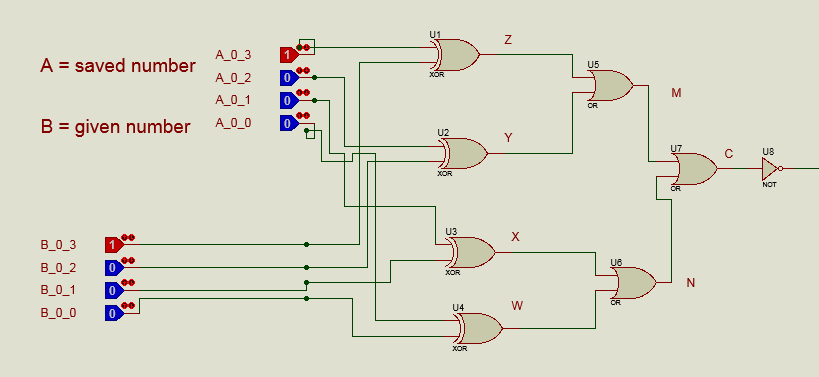
\includegraphics[width=1\textwidth]{diagram.png}
    \caption{\large Basic diagram of the lock system}
\end{figure}

\newpage
\section{Results and Analysis}

In this case, the stored digits(A) are 0001 and the input(B) given by a user
is also 0001. So, practically, this shoudl unlock the combinational lock. The process of figuring out whether
the stored and input values match or not is determined like so:

\vspace{1cm}

\begin{minipage}[t]{0.4\linewidth}
    \begin{center}
    \begin{tabular}{ |c|c| }
        \hline
        {\bf Stored Value} & {\bf Value}\\
        \hline
        A\_0\_0 & 0 \\
        \hline
        A\_0\_1 & 0 \\
        \hline
        A\_0\_2 & 0 \\
        \hline
        A\_0\_3 & 1 \\
        \hline
    \end{tabular}
    \end{center}
\end{minipage}\hfill
\begin{minipage}[t]{0.6\linewidth}
    \begin{center}
    \begin{tabular}{ |c|c| }
        \hline
        {\bf User Input} & {\bf Value}\\
        \hline
        B\_0\_0 & 0 \\
        \hline
        B\_0\_1 & 0 \\
        \hline
        B\_0\_2 & 0 \\
        \hline
        B\_0\_3 & 1 \\
        \hline
    \end{tabular}
    \end{center}
\end{minipage}

\vspace{1cm}

The values for the stored and inputs are fed accordingly into {\bf XOR Gates}
where their outputs are as the following:

\vspace{1cm}

\begin{minipage}[t]{0.5\linewidth}
    \begin{center}
        \begin{tabular}{ |c|c|c| }
            \hline
            {\bf A\_0\_0} & {\bf B\_0\_0} & {\bf W} \\
            \hline
            0 & 0 & 0\\
            \hline
        \end{tabular}
    \end{center}

    \vspace{.5cm}

    \begin{center}
        \begin{tabular}{ |c|c|c| }
            \hline
            {\bf A\_0\_1} & {\bf B\_0\_1} & {\bf X} \\
            \hline
            0 & 0 & 0\\
            \hline
        \end{tabular}
    \end{center}
\end{minipage}\hfill
\begin{minipage}[t]{0.5\linewidth}
    \begin{center}
        \begin{tabular}{ |c|c|c| }
            \hline
            {\bf A\_0\_2} & {\bf B\_0\_2} & {\bf Y} \\
            \hline
            0 & 0 & 0\\
            \hline
        \end{tabular}
    \end{center}
    \vspace{.5cm}
    \begin{center}
        \begin{tabular}{ |c|c|c| }
            \hline
            {\bf A\_0\_3} & {\bf B\_0\_3} & {\bf Z} \\
            \hline
            1 & 1 & 0\\
            \hline
        \end{tabular}
    \end{center}
\end{minipage}

\vspace{1cm}

The outputs from the XOR gates are then, fed into {\bf OR Gates} like so:

\vspace{1cm}

\begin{minipage}[t]{0.5\linewidth}
    \begin{center}
        \begin{tabular}{ |c|c|c| }
            \hline
            {\bf W} & {\bf X} & {\bf N} \\
            \hline
            0 & 0 & 0\\
            \hline
        \end{tabular}
    \end{center}
\end{minipage}\hfill
\begin{minipage}[t]{0.5\linewidth}
    \begin{center}
        \begin{tabular}{ |c|c|c| }
            \hline
            {\bf Y} & {\bf Z} & {\bf M} \\
            \hline
            0 & 0 & 0\\
            \hline
        \end{tabular}
    \end{center}
\end{minipage}

\vspace{1cm}

Then, the two outpus are input into another {\bf OR Gate},

\vspace{1cm}
\begin{center}
    \begin{tabular}{ |p{2cm}|p{2cm}|p{2cm}| }
        \hline
        \hfil {\bf M} & \hfil {\bf N} & \hfil {\bf C} \\
        \hline
        \hfil 0 & \hfil 0 & \hfil 0\\
        \hline
    \end{tabular}
\end{center}

\vspace{1cm}

Finally, the output from the last {\bf OR Gate} is fed into a {\bf NOT Gate} that determines whether the lock has been unlocked or not where an output of ``1'' indicates the combinational lock has been unlocked and ``0'' indicates it has not been unlocked.


\vspace{1cm}
\begin{center}
    \begin{tabular}{ |p{2cm}|p{3cm}| }
        \hline
        \hfil {\bf C} & \hfil {\bf NOT Gate} \\
        \hline
        \hfil 0 & \hfil 1 \\
        \hline
    \end{tabular}
\end{center}

\vspace{1cm}

Here, the final output from the {\bf NOT Gate} is ``1'' which indicates
that the stored digits and the user input digits are matching. However,
if there is any difference between the input and the stored values, one
of the {\bf XOR Gates} will have an output of ``1'' that at the end will
change the output of the final {\bf OR Gate} to ``1''. After this value
is fed into the final {\bf NOT Gate}, the final output will become ``0''
which means the lock has not been unlocked.

\vspace{.5cm}

The system can be expanded to accomodate even more digits by feeding
each output from the {\bf NOT Gates} into several {\bf AND Gates} where
the output will remain similar. This is recreated in our Proteus Project
file where we combined four individual systems into one single {\bf
Combinational Lock}. 

\vspace{1cm}

\section{Conclusion}

In this project we have tried to illustrate a 4 digit combinational lock system and if someone wants to input more than 4 digits, it is not possible. Therefore, it can be told that this project is not feasible and also should be used only as a prototype.







\end{document}

